%%%%%%%%%%%%%%%%%%don't forget if needed %%%%%%%%%%%%%%%%%%%%%
%\section[toc version]{title version%
%              \sectionmark{head version}}
%\sectionmark{head version}
%%%%%%%%%%%%%%%%%%%%%%%%%%%%%%%%%%%%%%%%%%%%%%%%%%%%%%%%%%%%%%
\def\titcourt{Melting-solidification cycle of a PCM with complete or parial melting}
\def\titlong{Melting-solidification cycle of a PCM with complete or parial melting}
%%%%%%%%%%%%%%%%%%%%%%%%%%%%%%%%%%%%%%%%%%%%%%%%%%%%%%%%%%%%%%%%
\chapter[\titlong]{\titlong%
              \chaptermark{\titcourt}}
\chaptermark{\titcourt}
\label{chap-SOLIDIFICATION}
%%%%%%%%%%%%%%%%%%%%%%%%%%%%%%%%%%%%%%%%%%%%%%%%%%%%%%%%%%%%%%%%
%%%%%%%%%%%%%%%%%%%%%%%%%%%%%%%%%%%%%%%%%%%%%%%%%%%%%%%%%%%%%%%%


\begin{figure}
	\begin{center}
		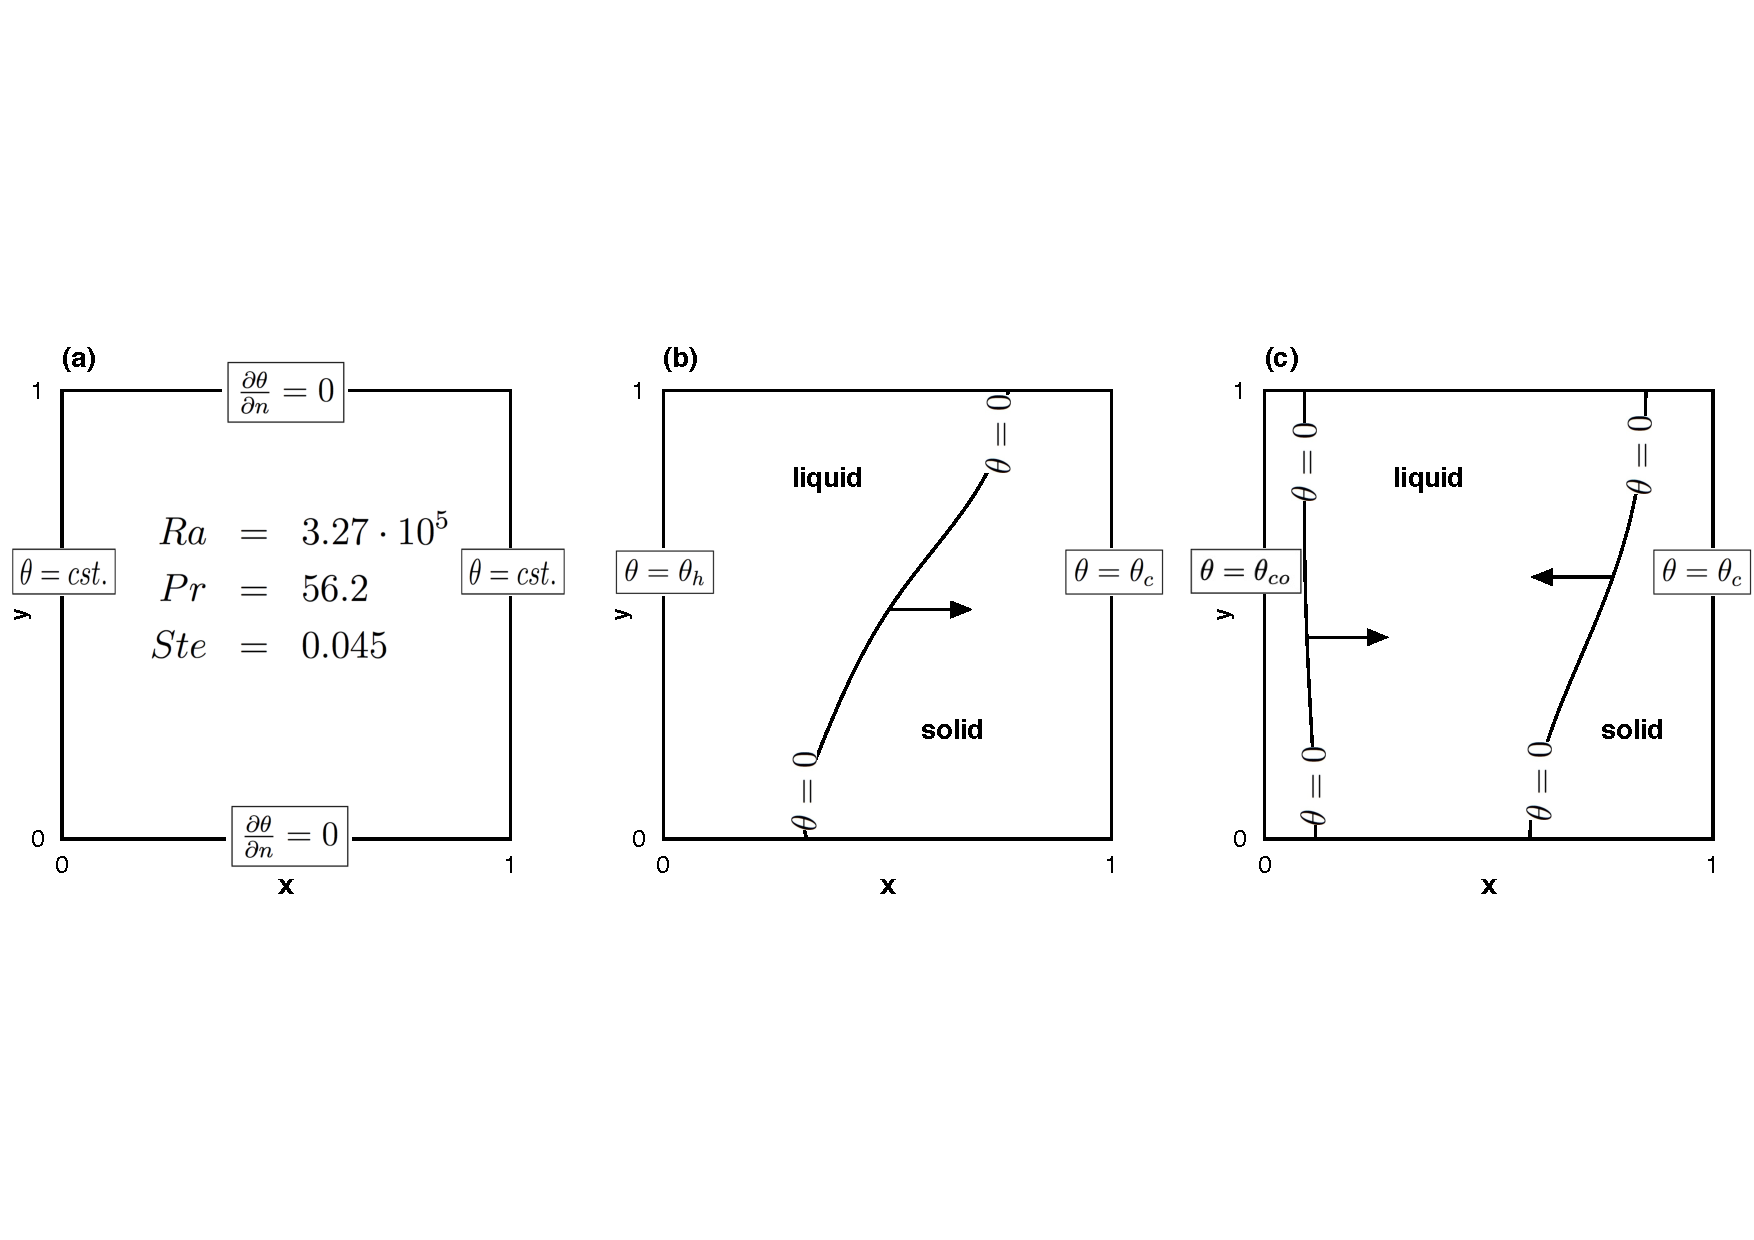
\includegraphics[width=\textwidth]{\figpath/Fig_cap_solidif/fig01_2}
	\end{center}
	\caption{Sketch of the computational domain and boundary conditions. General configuration (panel a) with isothermal ($\theta=cst.$) vertical ($x=0$ and $x=1$) walls and  adiabatic ($\partial \theta/\partial n = 0$) top and bottom walls. Configuration for the melting phase (panel b) with a hot left wall ($\theta=\theta_h > 0$) and a cold right wall ($\theta=\theta_c < 0$), followed by a solidification phase (panel c), when the temperature of the left wall is cooled to $\theta=\theta_{co} < 0$.}
	\label{fig: pcm-case}
\end{figure}

%\section{Solidification of the PCM}\label{sec: solidification-2D}
The fundamental operational mode of latent thermal energy storage (LTES) systems based on phase-change materials (PCM) is made of alternate melting and solidification cycles that  are not necessarily periodic. Partial melting and/or solidification of the PCM are often observed in applications and, in particular, in applications for buildings \citep{zhu2009dynamic,ascione2014energy}. 
The modern numerical approaches were mostly applied to simulate separately melting or solidification problems and only recently for alternate melting and solidification cycles \citep{wang2010numerical}. However, cyclic or periodic, melting and solidification problems have attracted considerable attention in the literature. \cite{ho1993periodic} and \cite{voller1996cyclic} studied numerically periodic melting in a square enclosure. Recently, \cite{hosseini2014experimental} presented experimental studies for the melting and the solidification of a cylindrical PCM during a charging and discharging process and \cite{chabot2017solid} studied analytically the effect of an alternate heating and cooling in a cylindrical PCM, with periodic boundary conditions. 
The present contribution is scoped  to offer an accurate numerical description of the alternate melting and solidification of a PCM.


After the melting of the PCM in Sec. \ref{chap-MELTING}, we present in this chapter the simulation of the solidification process.
The solidification of an octadecane PCM in a square cavity is considered.

\section{Numerical configuration and Non-dimensional parameter setting}
As emphasized previously,  the natural convection occurring in the melting PCM is driven by the temperature difference $\delta T = T_h - T_f$. The dimensionless number that depicts the ratio between the forces creating and those refraining motion, is the Rayleigh number, which appears in the dimensionless form of the Navier-Stokes equations with Boussinesq approximation (sec. \ref{chap-NSB}, eq. \ref{eq-Rayleigh}). The higher is its value, the more intense is the heat transfer.
Conversely, during the solidification, the phase-change is handled by the discharged temperature $T_{co}$, where the subscript 'co' stands for 'cooling'. In the geometry discussed in this chapter, this represents the temperature of the left wall. Thus, the relevant temperature difference in the solid phase of the PCM is $\delta T_{co} = T_f-T_{co}$ and the dimensionless temperature in the solid phase should be defined with respect to this $\delta T_{co}$. It is then obvious, for Eqs. (\ref{eq-Rayleigh}) and (\ref{eq-RePr}),  that the Rayleigh number should be defined using the same temperature difference.  However, because the Rayleigh number, as emphasized earlier, amounts for the motion created by hot temperature difference, we choose to keep the same definition for the Rayleigh number as for the melting case, still relevant for the melted core of the flow, where the persisting motion acts as a boundary condition for the solidification process.    
Under these conditions, in regard with the solidification process, we introduce  a new parameter,  $r_{\delta} = \delta T_{co}/(T_h-T_f)$, the normalised temperature is with respect to 
$T_f-T_{co}$ and the relevant Rayleigh number will then  $\Ray_{co}= r_{\delta} \times \Ray$, where $\Ray_{co}$ is the pseudo-Rayleigh number for solidification with a melted boundary. 
In the following, we will  describe  the process of solidification using three different values of $r_{\delta}$. 
A new scaling is moreover introduced: 
\begin{eqnarray}\label{ref-adimPCM2}
V_{ref}&=&\frac{\alpha_l}{H}  \, \Rightarrow  \, t = t_{\varphi} \frac{\, \nu_l }{ H^2 \, \Pr \,}\, \Rightarrow  \, \Rey  = \frac{1}{\Pr}.  \label{ref-adimdT} 
\end{eqnarray}
The solidification stage is indeed a slower process compared to the melting, therefore the use of an adapted scaling is more relevant.
This leads to a different time scaling for each cycle.

The sketch of the computational domain and boundary conditions are illustrated in Fig. \ref{fig: pcm-case}a, corresponding to the melting of octadecane PCM presented in Sec. \ref{sec: melting-2D}.
Starting from a melting PCM (Fig. \ref{fig: pcm-case}b), the simulation of the solidification process starts by imposing at the left-wall a constant (cold) temperature $\theta_{co}$ as it is shown in Fig. \ref{fig: pcm-case}c.
We consider two cases: \\ 
-- case CM: solidification after a Complete Melting of the material ($L_f=0.95$, Figure \ref{fig:melt-field}f) and \\
-- case PM: solidification after a Partial Melting ($L_f=0.5$, Figure \ref{fig:melt-field}d). \\
 The solid phase will propagate into the cavity from both left and right sides  (Fig. \ref{fig: pcm-case}c), which makes this case computationally challenging. The mesh adaptivity capabilities of our numerical code made possible to accurately track the 
two solidification fronts identified by the iso-line $\theta=0$.  
In the discussion below,  the solidification process starts at physical time $t_{\varphi} = 185 $ min (corresponding to $\tau=0.2$) for case CM and at $t_{\varphi} = 59$ min ($\tau=0.06$) for case PM. 

\section{Solidification after a complete melting. Case CM.} \label{sec_solid_full} 

\begin{figure}
	\begin{center}
		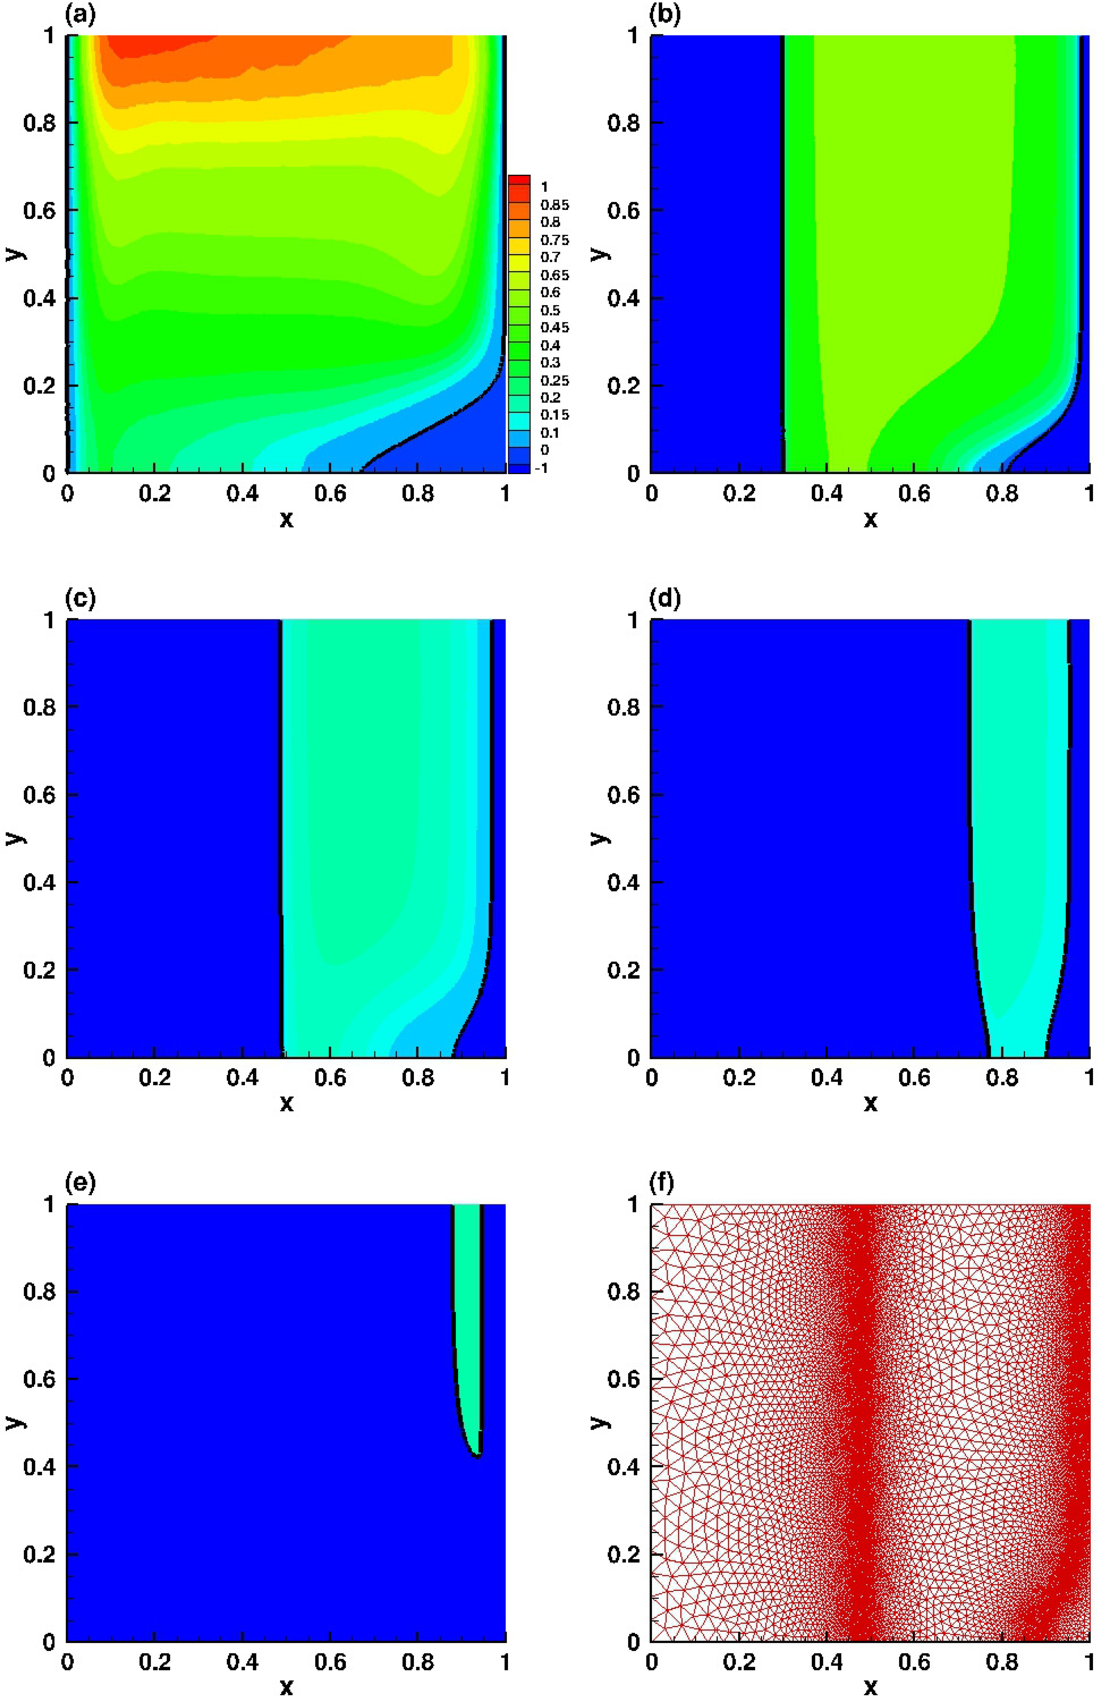
\includegraphics[width=.85\textwidth]{\figpath/Fig_cap_solidif/fig10}
	\end{center}
	\caption{Solidification of the PCM after a complete melting. 
	Temperature iso-lines in the liquid phase. 
	The solid part is represented in blue and corresponds to the region of temperature $\theta_{co} \leq \theta_f=0$. 
	Time instants (panels  a to e): $t_{\varphi} = 185$ min, $t_{\varphi} = 231$ min, $t_{\varphi} = 300$ min, $t_{\varphi} = 430$ min and $t_{\varphi} = 510$ min. 
	The adapted mesh corresponding to $t_{\varphi} = 300$ min is plotted in panel (f).  $\Ray_{co}=3.27 \cdot 10^5$. }\label{fig:evolution}
\end{figure}

The simulation continues from the state corresponding to Figure  \ref{fig:melt-field} at $t_{\varphi} =185$ min ($\tau=0.063$) and solidification follows after a complete melting. 
 Figure \ref{fig:evolution} shows the evolution of the PCM during the solidification process. At  $t_{\varphi}  =185$ min     (Figure \ref{fig:evolution}a), the liquid fraction is $L_f=0.95$ and the melting/solidification front is close to the right wall of the cavity. Setting a low temperature $\theta_{co} = -1$ at the left wall, while the right wall is maintained at a constant temperature ($\theta_{right} = -0.01 \leq \theta_f$) triggers the formation of a second solidification front, propagating from the left side of the domain. 
Figures \ref{fig:evolution}b and \ref{fig:evolution}c illustrate the left part of the cavity solidifying at a faster rate because of the very low temperature imposed at the left wall, inducing a non symmetric evolution of the solid-liquid interfaces.
The solid part is represented in blue and corresponds to the region of temperature $\theta \leq 0$.
The signature of the conductive heat transfer is characterized by the vertical shape of the left front.
Inside the liquid, the initial convection cells facilitate the heat transfer from the boundaries, resulting in a very rapid decrease of the fluid temperature. 
Temperature gradients being smoothed out during this first stage, the influence of the convection inside the liquid region is considerably reduced. As a result, the velocity inside the liquid is reduced to very low values. 
From $t_{\varphi} = 430$ min (Figure \ref{fig:evolution}d), the shape of both interfaces is almost symmetrical. 
This is a signature of a conduction dominated process. 
At $t_{\varphi} = 510$ min (Figure \ref{fig:evolution}e) the liquid region starts to shrink at the bottom side of the cavity. This process is accelerated and finally the liquid is trapped in a thin pocket and disappears completely through the top of the cavity (Figure \ref{fig:evolution}e). The complete solidification ends at $t_{\varphi} = 530$ min, \ie the liquid fraction is $L_f=0$.  
The adapted mesh, refined along the two solidification fronts, at $t_{\varphi} = 300$ min is reported in Figure \ref{fig:evolution}f, illustrating the efficiency of the adaptive mesh tool.


\section{Solidification after a partial melting. Case PM.} \label{sec_solid_partial} 

In this case, the solidification starts from the state corresponding to Figure \ref{fig:evolution_t80}a at $t_{\varphi} = 59$ min ($\tau=0.032$), when the liquid fraction is $L_f = 0.5$. 
The temperature of the left wall is suddenly lower at $\theta_{co}=-1$ as in the previous solidification simulation.  
The time evolution of the process is illustrated in Figures \ref{fig:evolution_t80}a-e, while the adapted mesh corresponding to $t_{\varphi} = 90$ min is plotted in Figure \ref{fig:evolution_t80}f. 
As in the previous case, a second  solidification front starts to propagate from the left side of the cavity. 
The straight shape of the left solid front is always observed while the right solid front is impacted by the convection cell present in the central liquid region (Figure \ref{fig:evolution_t80}b). 
The stronger convective effect is most likely due to the huge temperature difference that occurs over a smaller space distance (almost half of the volume is occupied by the solid state). 
This leads to stronger temperature gradients in the liquid region, and consequently to a stronger heat transfer.   
The two fronts merge to form a pocket of fluid which is connected to the top of the cavity (Figure \ref{fig:evolution_t80}c-e). 
It is interesting to  note that, as in the previous solidification case, the left part is solidifying at a faster rate, hence the pocket of melted PCM disappears completely from the right at the top side of the cavity (Figures \ref{fig:evolution_t80}c-e).
\begin{figure}
	\begin{center}
		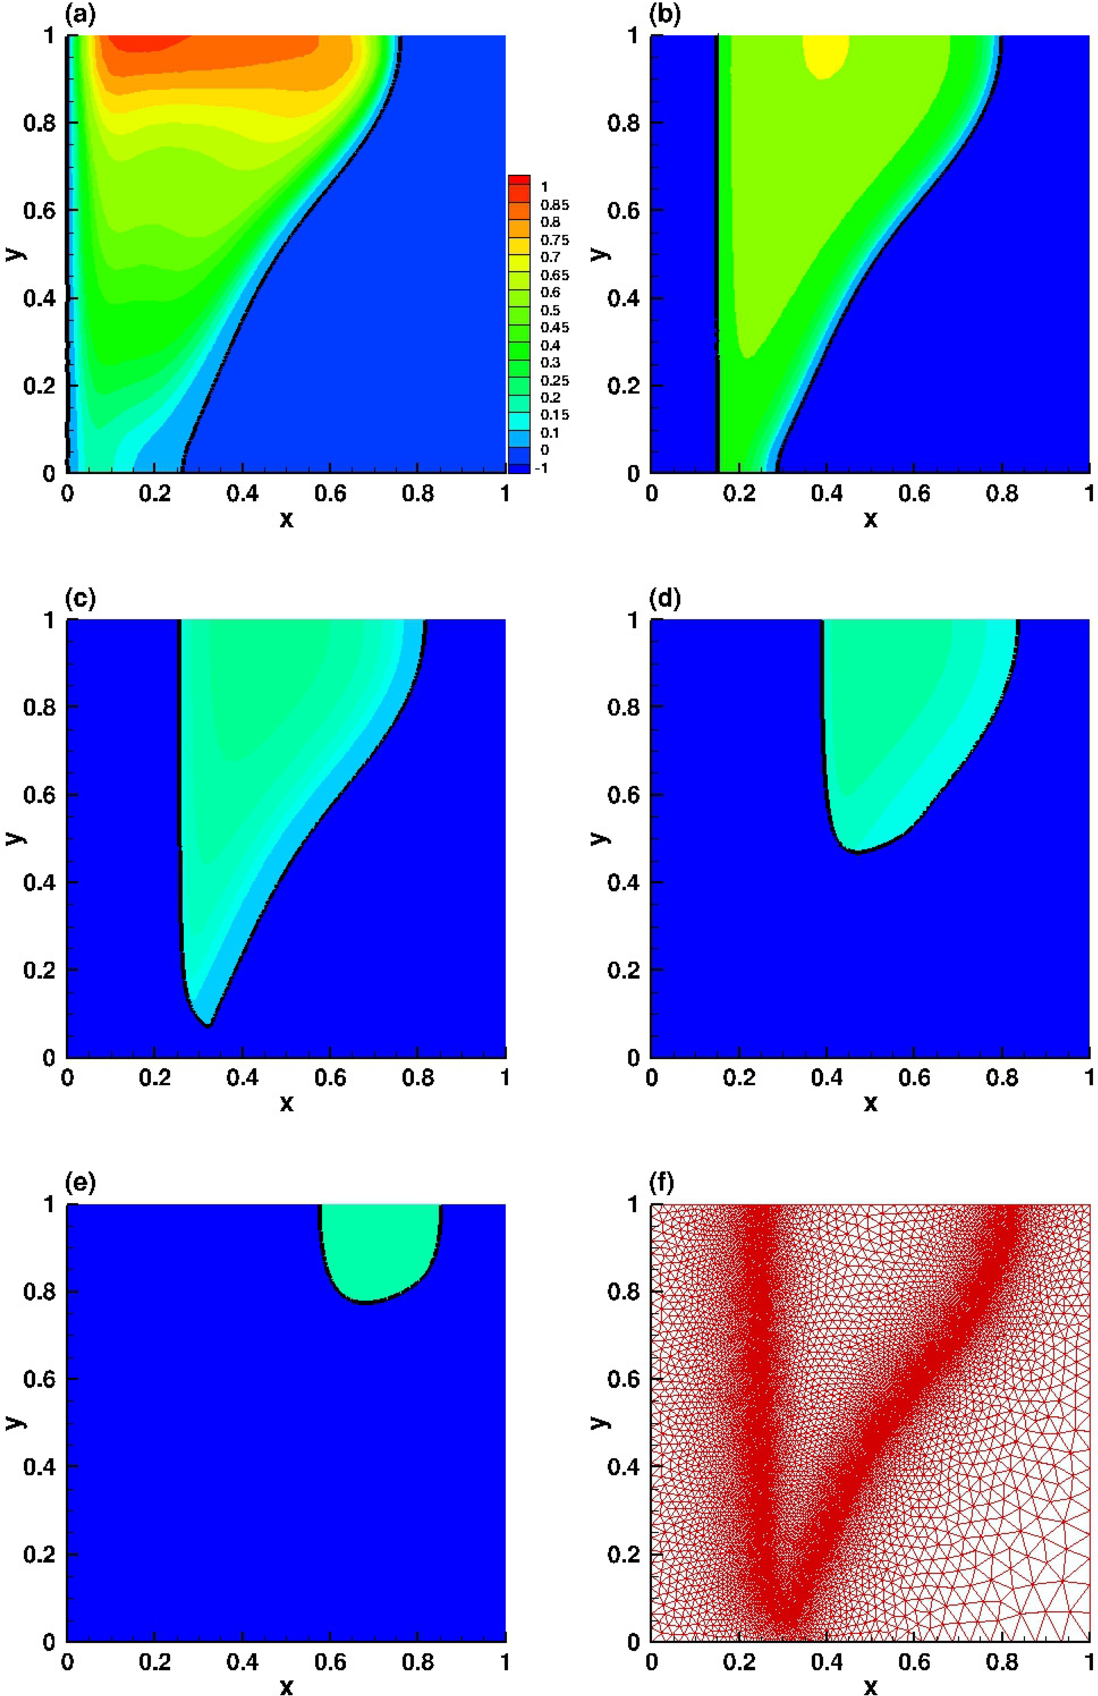
\includegraphics[width=.85\textwidth]{\figpath/Fig_cap_solidif/fig11}
	\end{center}
	\caption{Solidification of the PCM after a partial melting. Temperature iso-lines in the liquid phase. The solid part is represented in blue and corresponds to the region of temperature $\theta_{co} \leq \theta_f=0$. Time instants (panels  a to e): $t_{\varphi} = 59$ min, $t_{\varphi} = 70$ min, $t_{\varphi} = 90$ min, $t_{\varphi} = 131$ min and $t_{\varphi} = 200$ min. The adapted mesh corresponding to $t_{\varphi} = 90$ min is plotted in panel (f).  $ \Ray_{co}=3.27 \cdot 10^5$.}\label{fig:evolution_t80}
\end{figure}

\section{Analysis of the solidification cycle from two different initial conditions: complete and partial melting. Cases CM and PM. } \label{sec_freezing_full} 

The aim of this subsection is to investigate the temporal evolution of some physical properties of the solidification process, from two different initial conditions: i) completely melted volume (case CM) and ii) partially melted volume ($50\%$ of the fluid is melted, case PM).  
 
Figure \ref{fig:Lf_full_1D_profil} represents the temporal  evolution of the liquid fraction, note that the average Nusselt number is calculated at the cooled wall defined similarly to (\ref{eq-Nu}) but it can be negative in this case and the accumulated heat input $Q_0$, for the two investigated cases. $Q_0$ is defined as follows:
\begin{equation}
    Q_0 = \int_0^{t_{\varphi}} N\!u \, d t_{\varphi},
    \label{eq-Q0}
\end{equation}

\Blue{
Simulations for three values $r_{\delta} = 1$,  $r_{\delta} = 5$ and  $r_{\delta} = 10$ are carried out.
}

Figure \ref{fig:Lf_full_1D_profil}(a) illustrates the temporal evolution of the liquid fraction $L_f$ for the CM case. 
Complete melting occurs for $t_{\varphi} =185$ min, after which solidification starts, with a continuous decrease of $L_f$ till complete solidification is achieved. 
For the lowest value of \Blue{$r_{\delta}$, corresponding to $\Ray_{co} = 3.27 \cdot 10^5$}, the solidification process ends at $t_{\varphi} = 530$ min. 
Then, the higher value of \Blue{$r_{\delta}$}, the faster the discharge process,
with final times $t_{\varphi} = 260$ min and $t_{\varphi} = 230$ min for cases \Blue{$\Ray_{co} = 1.62 \cdot 10^6$} and \Blue{$ \Ray_{co} = 3.27 \cdot 10^6$}, i.e. a drop of the cold boundary temperature by a factor of 5 and 10 respectively.
The solidification speed, quantified by $d L_f/ d t_{\varphi}$ is  nearly constant during almost the whole process for each case.  
This uniformity of the process indicates that the natural convection flow vanishes during the solidification, and conduction remains the only heat transfer mode.   

Figure \ref{fig:Lf_full_1D_profil}(b) plots the temporal evolution of $L_f$ for the PM case. 
As previously discussed, $50\%$ of the volume is melted, at time $t_{\varphi} = 59$ min, then solidification starts. 
Furthermore, noticeable is that, despite that solidification process is started, $L_f$ continues to increase slightly at the very beginning of the discharge stage, and then decreases monotonically towards $0$ at $t_{\varphi} = 240$ min.
The heat stored in the melted PCM continues to melt the remaining solid PCM until the convection becomes negligible.
It is worth noticing that this behavior is not observed in the complete melting case because of the imposed temperature at the right wall.  


\begin{figure}[!h]
\begin{center}
\begin{minipage}[t]{0.7\textwidth}
	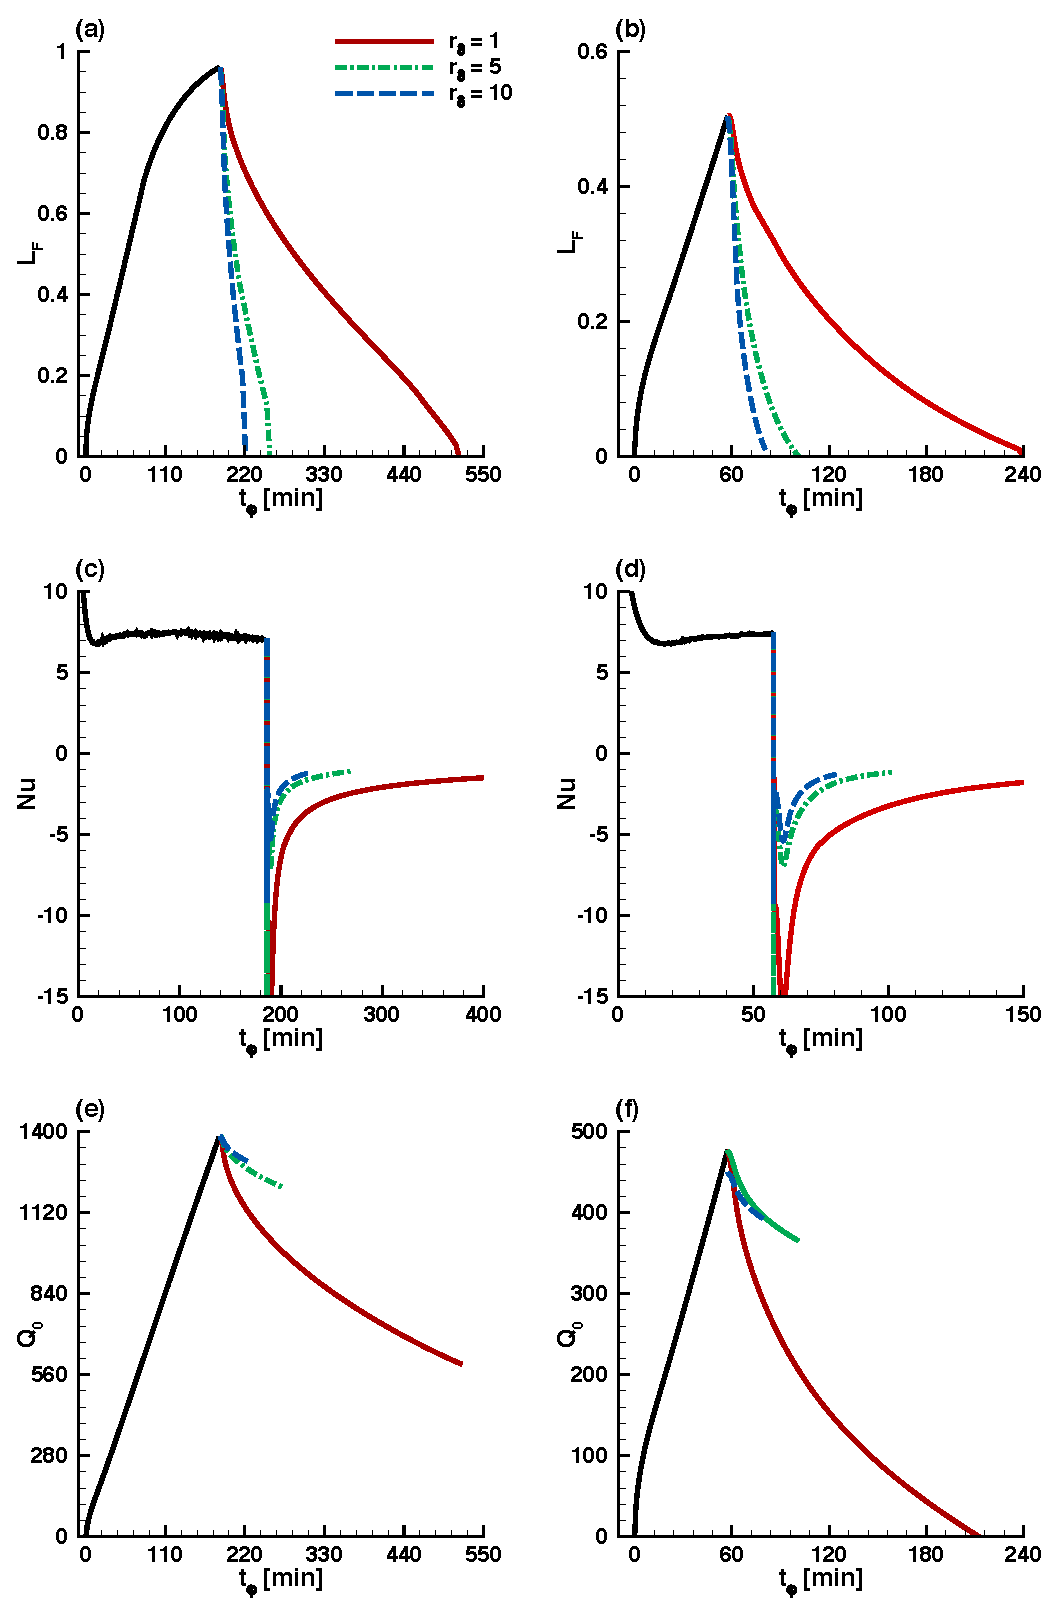
\includegraphics[width=\textwidth]{\figpath/Fig_cap_solidif/fig12_3}
\end{minipage}
\end{center}
\caption{Temporal evolution of the  liquid fraction ($L_f$), the Nusselt number $N\!u$, and the accumulated heat input $Q_0$ during the entire melting-solidification cycle. Case CM  (left) and  case PM  (right).}\label{fig:Lf_full_1D_profil}
\end{figure}

Let us now pay attention to the transfers occurring at the left wall, suddenly submitted to a lower temperature. This is done through the temporal evolution of the Nusselt number,  and the temporal-integrated values of the Nusselt number, or the accumulated heat input.     

Panels (c) and (d) of the Figure \ref{fig:Lf_full_1D_profil} illustrate the Nusselt number for the CM and PM.  
The three investigated Rayleigh numbers are shown, with clear differences between them. This difference corroborates with that already reported for the melting case, over shorter times scales.   This indicates that the heat transfer during the solidification process is fundamentally different from the melting one.

For the CM case, for \Blue{$\Ray_{co}=3.27 \cdot 10^5$,  the Nusselt number first decreases sharply, for  $t_{\varphi} \leq 18$ min, then it reaches a plateau at $N\!u=7$ during the complete melting. At $t_{\varphi}=185$ min, solidification starts and $N\!u$ suddenly decreases over very short times, reaching negative values ($N\!u\approx -15$). It follows an increase of $N\!u$ with time, up to reaching an asymptotic value close to $0$ (zero temperature gradients, i.e. uniform temperature at the left wall).  
The same mechanism is observed over a shorter time interval when} \Blue{$\Ray_{co}$} is increased.

For the PM case, the Nusselt number also decreases sharply to a negative value when the solidification starts.
However, the convection flow remaining in the melted region influences the heat transfer at the very beginning of the solidification process.
The hot fluid in the middle of the melted PCM is advected by the natural convection flow to the boundaries and induces a temperature gradient at the left wall, resulting into an oscilating behavior of the Nusselt number before reaching asymptotic value.
This is in agreement with the previous comment about the melting continuing in the right part of the cavity, despite the solidification has started, and the slight increase of the liquid fraction at the very first time steps of the discharging process.


Both charge and  discharge cycles are better illustrated in the time evolution of the accumulated heat $Q_0$ defined in (\ref{eq-Q0}), as it is shown in panels (d) and (e) of Figure  \ref{fig:Lf_full_1D_profil}.
Heat is first stored during the melting stage, corresponding to $t_{\varphi} \leq 185$ min for CM (Figure \ref{fig:Lf_full_1D_profil}(d)) and $\tau \leq 59$ min for PM (Figure \ref{fig:Lf_full_1D_profil}(e)), and is then restored during the solidification stage.

\noindent The CM case indicates higher value of $Q_0$ ($Q_0 = 1400$, for \Blue{$\Ray_{co} = 3.27 \cdot 10^5$) compared to the PM case ($Q_0 = 500$), meaning that PCM is more efficient in terms of heat storage.
However, PM case exhibits well balanced characteristic times between the solidification and the melting stages for} \Blue{$\Ray_{co} = 3.27 \cdot 10^5$.}
Besides, when the Ra number increases, the stored heat is discharged faster.

\noindent Moreover, the temperature and the velocity profiles drop sharply during the first step of the cooling process and become almost equal to zero very early in the whole domain.
This means that conduction dominates the solidification process, and the convection becomes rapidly negligible.
As a consequence, the melting fronts are vertical and have a symmetric position with respect to the center of the cavity. \\
